% Options for packages loaded elsewhere
\PassOptionsToPackage{unicode}{hyperref}
\PassOptionsToPackage{hyphens}{url}
%
\documentclass[
]{book}
\usepackage{lmodern}
\usepackage{amssymb,amsmath}
\usepackage{ifxetex,ifluatex}
\ifnum 0\ifxetex 1\fi\ifluatex 1\fi=0 % if pdftex
  \usepackage[T1]{fontenc}
  \usepackage[utf8]{inputenc}
  \usepackage{textcomp} % provide euro and other symbols
\else % if luatex or xetex
  \usepackage{unicode-math}
  \defaultfontfeatures{Scale=MatchLowercase}
  \defaultfontfeatures[\rmfamily]{Ligatures=TeX,Scale=1}
\fi
% Use upquote if available, for straight quotes in verbatim environments
\IfFileExists{upquote.sty}{\usepackage{upquote}}{}
\IfFileExists{microtype.sty}{% use microtype if available
  \usepackage[]{microtype}
  \UseMicrotypeSet[protrusion]{basicmath} % disable protrusion for tt fonts
}{}
\makeatletter
\@ifundefined{KOMAClassName}{% if non-KOMA class
  \IfFileExists{parskip.sty}{%
    \usepackage{parskip}
  }{% else
    \setlength{\parindent}{0pt}
    \setlength{\parskip}{6pt plus 2pt minus 1pt}}
}{% if KOMA class
  \KOMAoptions{parskip=half}}
\makeatother
\usepackage{xcolor}
\IfFileExists{xurl.sty}{\usepackage{xurl}}{} % add URL line breaks if available
\IfFileExists{bookmark.sty}{\usepackage{bookmark}}{\usepackage{hyperref}}
\hypersetup{
  pdftitle={Relazione di tesi:  La serie di Fourier  e una sua applicazione alla grafica},
  pdfauthor={Matteo Bramardi, candidato; Prof.~Paolo Boggiatto, relatore},
  hidelinks,
  pdfcreator={LaTeX via pandoc}}
\urlstyle{same} % disable monospaced font for URLs
\usepackage{color}
\usepackage{fancyvrb}
\newcommand{\VerbBar}{|}
\newcommand{\VERB}{\Verb[commandchars=\\\{\}]}
\DefineVerbatimEnvironment{Highlighting}{Verbatim}{commandchars=\\\{\}}
% Add ',fontsize=\small' for more characters per line
\usepackage{framed}
\definecolor{shadecolor}{RGB}{248,248,248}
\newenvironment{Shaded}{\begin{snugshade}}{\end{snugshade}}
\newcommand{\AlertTok}[1]{\textcolor[rgb]{0.94,0.16,0.16}{#1}}
\newcommand{\AnnotationTok}[1]{\textcolor[rgb]{0.56,0.35,0.01}{\textbf{\textit{#1}}}}
\newcommand{\AttributeTok}[1]{\textcolor[rgb]{0.77,0.63,0.00}{#1}}
\newcommand{\BaseNTok}[1]{\textcolor[rgb]{0.00,0.00,0.81}{#1}}
\newcommand{\BuiltInTok}[1]{#1}
\newcommand{\CharTok}[1]{\textcolor[rgb]{0.31,0.60,0.02}{#1}}
\newcommand{\CommentTok}[1]{\textcolor[rgb]{0.56,0.35,0.01}{\textit{#1}}}
\newcommand{\CommentVarTok}[1]{\textcolor[rgb]{0.56,0.35,0.01}{\textbf{\textit{#1}}}}
\newcommand{\ConstantTok}[1]{\textcolor[rgb]{0.00,0.00,0.00}{#1}}
\newcommand{\ControlFlowTok}[1]{\textcolor[rgb]{0.13,0.29,0.53}{\textbf{#1}}}
\newcommand{\DataTypeTok}[1]{\textcolor[rgb]{0.13,0.29,0.53}{#1}}
\newcommand{\DecValTok}[1]{\textcolor[rgb]{0.00,0.00,0.81}{#1}}
\newcommand{\DocumentationTok}[1]{\textcolor[rgb]{0.56,0.35,0.01}{\textbf{\textit{#1}}}}
\newcommand{\ErrorTok}[1]{\textcolor[rgb]{0.64,0.00,0.00}{\textbf{#1}}}
\newcommand{\ExtensionTok}[1]{#1}
\newcommand{\FloatTok}[1]{\textcolor[rgb]{0.00,0.00,0.81}{#1}}
\newcommand{\FunctionTok}[1]{\textcolor[rgb]{0.00,0.00,0.00}{#1}}
\newcommand{\ImportTok}[1]{#1}
\newcommand{\InformationTok}[1]{\textcolor[rgb]{0.56,0.35,0.01}{\textbf{\textit{#1}}}}
\newcommand{\KeywordTok}[1]{\textcolor[rgb]{0.13,0.29,0.53}{\textbf{#1}}}
\newcommand{\NormalTok}[1]{#1}
\newcommand{\OperatorTok}[1]{\textcolor[rgb]{0.81,0.36,0.00}{\textbf{#1}}}
\newcommand{\OtherTok}[1]{\textcolor[rgb]{0.56,0.35,0.01}{#1}}
\newcommand{\PreprocessorTok}[1]{\textcolor[rgb]{0.56,0.35,0.01}{\textit{#1}}}
\newcommand{\RegionMarkerTok}[1]{#1}
\newcommand{\SpecialCharTok}[1]{\textcolor[rgb]{0.00,0.00,0.00}{#1}}
\newcommand{\SpecialStringTok}[1]{\textcolor[rgb]{0.31,0.60,0.02}{#1}}
\newcommand{\StringTok}[1]{\textcolor[rgb]{0.31,0.60,0.02}{#1}}
\newcommand{\VariableTok}[1]{\textcolor[rgb]{0.00,0.00,0.00}{#1}}
\newcommand{\VerbatimStringTok}[1]{\textcolor[rgb]{0.31,0.60,0.02}{#1}}
\newcommand{\WarningTok}[1]{\textcolor[rgb]{0.56,0.35,0.01}{\textbf{\textit{#1}}}}
\usepackage{longtable,booktabs}
% Correct order of tables after \paragraph or \subparagraph
\usepackage{etoolbox}
\makeatletter
\patchcmd\longtable{\par}{\if@noskipsec\mbox{}\fi\par}{}{}
\makeatother
% Allow footnotes in longtable head/foot
\IfFileExists{footnotehyper.sty}{\usepackage{footnotehyper}}{\usepackage{footnote}}
\makesavenoteenv{longtable}
\usepackage{graphicx,grffile}
\makeatletter
\def\maxwidth{\ifdim\Gin@nat@width>\linewidth\linewidth\else\Gin@nat@width\fi}
\def\maxheight{\ifdim\Gin@nat@height>\textheight\textheight\else\Gin@nat@height\fi}
\makeatother
% Scale images if necessary, so that they will not overflow the page
% margins by default, and it is still possible to overwrite the defaults
% using explicit options in \includegraphics[width, height, ...]{}
\setkeys{Gin}{width=\maxwidth,height=\maxheight,keepaspectratio}
% Set default figure placement to htbp
\makeatletter
\def\fps@figure{htbp}
\makeatother
\setlength{\emergencystretch}{3em} % prevent overfull lines
\providecommand{\tightlist}{%
  \setlength{\itemsep}{0pt}\setlength{\parskip}{0pt}}
\setcounter{secnumdepth}{5}
\usepackage{booktabs}
\usepackage[]{natbib}
\bibliographystyle{plainnat}

\title{Relazione di tesi: La serie di Fourier e una sua applicazione alla grafica}
\author{Matteo Bramardi, candidato \and Prof.~Paolo Boggiatto, relatore}
\date{A.A. 2019/2020}

\begin{document}
\maketitle

{
\setcounter{tocdepth}{1}
\tableofcontents
}
\hypertarget{introduzione}{%
\chapter*{Introduzione}\label{introduzione}}
\addcontentsline{toc}{chapter}{Introduzione}

L'idea per l'argomento della tesi nasce dal video \href{https://www.youtube.com/watch?v=r6sGWTCMz2k}{\emph{But what is a Fourier series? From heat flow to circle drawings}} pubblicato su YouTube da Grant Sanderson, noto come \href{https://www.youtube.com/c/3blue1brown}{\emph{\textbf{3Blue1Brown}}}. Rimasto colpito dal fascino estetico delle animazioni e dalla loro squisita immediatezza, ho deciso di approfondirne i fondamenti teorici.

Il cuore della tesi è la \href{https://bradwave.github.io/thesis}{\textbf{presentazione}} che, oltre ad una dissertazione teorica del tema, ripropone le suddette \textbf{animazioni}, da me ricreate ed adattate. La presentazione è affinata per agevolarne la comprensione attraverso l'\textbf{interazione} con diversi suoi elementi e aspira ad essere un esempio di applicazione delle tecnologie informatiche a fini didattici.

Essa è il risultato di quasi un anno di lavoro e studio personale e concretizza la mia idea di presentare la matematica in modo \textbf{coinvolgente} e con l'ausilio di \textbf{visualizzazioni grafiche} di forte impatto e semplice interpretazione.

\hypertarget{lavoro}{%
\chapter{Fasi del lavoro}\label{lavoro}}

\hypertarget{prototipi}{%
\section{Primi prototipi}\label{prototipi}}

Dopo la visione del \href{https://www.youtube.com/watch?v=r6sGWTCMz2k}{video sopracitato} nel mese di luglio 2019, ho realizzato il primo prototipo dell'animazione principale in \emph{JavaScript} seguendo \href{https://www.youtube.com/watch?v=MY4luNgGfms}{alcuni tutorial} di \href{https://www.youtube.com/thecodingtrain}{\emph{The Coding Train}}. A dicembre dello stesso anno ho poi riscritto il precedente prototipo in \emph{Java} e ne ho ampliato le funzionalità. Ciò mi ha permesso di familiarizzare con i vari algoritmi impiegati nella generazione delle informazioni utili alla visualizzazione dell'animazione e con la loro implementazione.

\hypertarget{ricerca}{%
\section{Ricerca teorica}\label{ricerca}}

Già nel mese di dicembre 2019 mi ero approcciato allo studio della trasformata di Fourier e di una sua applicazione alla compressione delle immagini con il metodo JPEG \emph{lossy} - basato sulla trasformata discreta del coseno - con lo scopo di produrre un \href{https://bradwave.myportfolio.com/the-fourier-transform}{trittico di poster} sull'argomento, parte della prova di esame del corso di \emph{Analisi Matematica 3}.

La fase di ricerca teorica vera e propria ha avuto inizio nel mese di marzo 2020 e, su indicazione del mio relatore Prof.~Paolo Boggiatto, ha riguardato principalmente lo studio approfondito di alcune sezioni del libro \emph{\textbf{Fourier Analysis and Applications}} di C. Gasquet e P. Witomski: nello specifico, il capitolo II - \emph{i segnali periodici e la serie di Fourier} -, la lezione 8 del capitolo III - \emph{la trasformata discreta di Fourier} - e le lezioni 17, 18 e 19 del capitolo VI - \emph{la trasformata di Fourier di funzioni integrabili, la trasformata inversa e lo spazio \(\mathcal{S}(\mathbb{R})\)}.

La questione centrale della tesi, alla base del funzionamento dell'animazione, riguarda la possibilità di scrivere una funzione \(f: \mathbb{R} \longrightarrow \mathbb{C}\) periodica di periodo \(a\) come
\[f(t)=\sum_{n=-\infty}^{+\infty}c_{n}e^{2\pi in \frac{t}{a}} \ ,\]
dove \(c_n \in \mathbb{C}\) e \(n \in \mathbb{Z}\), sotto \emph{minime ipotesi} sulla funzione \(f\).

Inoltre, durante lo sviluppo del software, si è rivelato utile affrontare il tema delle curve di Bèzier, in particolare delle \emph{polybézier} - ovvero di una curva di Bèzier continua definita a tratti. Per potenziare le mie conoscenze in materia, ho fatto uso del libro \emph{A Primer on Bézier Curves}, \href{https://pomax.github.io/bezierinfo/}{disponibile online}, che mi ha fornito le basi necessarie per manipolare tali oggetti da un punto di vista informatico.

Prima della fase di programmazione si è poi resa necessaria una ricerca degli strumenti informatici più adatti. Una discussione degli strumenti adottati e del loro impiego è consultabile al \protect\hyperlink{software}{capitolo dedicato}.

\hypertarget{animazioni}{%
\section{Animazioni}\label{animazioni}}

Terminata la raccolta e lo studio delle informazioni necessarie, ha potuto avere inizio la programmazione delle animazioni in maniera più accurata rispetto ai \protect\hyperlink{prototipi}{primi prototipi}.
Il loro sviluppo è avvenuto in \emph{JavaScript}, facendo ampio uso delle librerie \emph{open source} \href{https://p5js.org/}{\emph{p5.js}}, per il \emph{creative coding}, e \href{https://github.com/infusion/Complex.js/}{\emph{complex.js}}, per la gestione dei numeri complessi. Ciò ha permesso, a differenza di un semplice video, di rendere le animazioni \textbf{interattive}, andando così a potenziare il legame con lo spettatore che si trasforma quindi in \textbf{utente attivo}.

L'obiettivo delle animazioni è quello di agevolare la comprensione dei concetti teorici tramite una loro \textbf{visualizzazione immediata} e metterne in evidenza le sfaccettature più nascoste, andando ad affiancare ed assistere l'ingegno e le capacità immaginative dei loro fruitori.

Molta attenzione è stata riposta nella loro \textbf{estetica}, in quanto ritengo che l'aspetto artistico non sia affatto secondario al contenuto, ma piuttosto funzionale a quest'ultimo, poiché in grado di avvicinare e coinvolgere lo spettatore-utente instaurando una connessione emotiva e sensoriale più forte.
La filosofia alla base di questo approccio deriva sicuramente dalla visione artistica del \href{https://www.youtube.com/watch?v=r6sGWTCMz2k}{video originale}. Tuttavia, è stata ampiamente influenzata anche dagli \emph{Elementi} di Euclide a colori, ovvero un'edizione del celebre libro di geometria in cui simboli e figure colorate sostituiscono le lettere, e dal pensiero del suo autore, Oliver Byrne, che ho avuto modo di apprezzare durante il corso di \emph{Storia della Matematica Antica e Moderna}.

Ho infine curato l'\textbf{accessibilità}, ovvero la facilità di utilizzo, e la \textbf{portabilità}, cioè la corretta visualizzazione e fruizione su diversi tipi di dispositivi, principi chiavi per garantire all'utente un'esperienza fluida e priva di ostacoli o barriere di carattere tecnico.

\hypertarget{presentazione}{%
\section{Presentazione}\label{presentazione}}

La presentazione è stata realizzata con \href{https://revealjs.com/}{\emph{\textbf{Reveal.js}}}, un framework \emph{open source} per presentazioni HTML a cui ho apportato diverse personalizzazioni.
Ciò mi ha permesso di \textbf{integrare perfettamente} (ovvero \emph{seamlessly} in inglese) le \textbf{animazioni} nell'ambiente della presentazione, senza richiedere all'utente operazioni aggiuntive. Inoltre, il file HTML può essere visualizzato da un'ampia gamma di dispositivi tramite un qualsiasi \emph{browser} e le ridotte dimensioni del file lo rendono ideale per la distribuzione online.

\hypertarget{filosofia}{%
\subsubsection*{}\label{filosofia}}
\addcontentsline{toc}{subsubsection}{}

La filosofia che mi ha guidato nella creazione delle slide è la stessa discussa nel \protect\hyperlink{animazioni}{precedente paragrafo}: accessibilità e piacevolezza estetica hanno costituito il fondamento su cui sviluppare il contenuto e il mezzo con cui esaltarlo, ma senza in alcun modo prevaricarlo. In tal senso, \protect\hyperlink{features}{diversi accorgimenti} sono stati adottati per affinare l'esperienza dell'utente finale.

\hypertarget{section}{%
\subsubsection*{}\label{section}}
\addcontentsline{toc}{subsubsection}{}

Nel \protect\hyperlink{commento}{capitolo successivo} verrà fornito un commento di carattere teorico alla presentazione.

\hypertarget{commento}{%
\chapter{Commento alla presentazione}\label{commento}}

La presentazione segue per sommi capi le prime due lezioni del \textbf{capitolo II} del libro \emph{\textbf{Fourier Analysis and Applications}} di C. Gasquet e P. Witomski, oggetto della \protect\hyperlink{ricerca}{ricerca}. Le slide sono autonome da un punto di vista teorico e possono essere utilizzate parallelamente al libro sopracitato come strumento supplementare per l'apprendimento.

\hypertarget{features}{%
\subsection*{Funzionalità}\label{features}}
\addcontentsline{toc}{subsection}{Funzionalità}

\begin{itemize}
\tightlist
\item
  Le animazioni sono \textbf{integrate} nella presentazione ed è possibile \textbf{interagire} con esse;
\item
  formule, teoremi (o corollari) ed esempi sono demarcati rispettivamente con colore azzurro, verde e giallo per un più \textbf{semplice riconoscimento};
\item
  formule e teoremi vengono visualizzati in una piccola scheda al passaggio o click del mouse sui rispettivi riferimenti, rendendo \textbf{immediata} la loro \textbf{consultazione}, mentre un ulteriore click su tali schede conduce alla slide in cui sono stati introdotti;
\end{itemize}

\hypertarget{segntrig}{%
\section{Segnali trigonometrici}\label{segntrig}}

Diciamo \emph{\textbf{polinomi trigonometrici}} le funzioni del tipo

\begin{equation}
  p(t) = \sum_{n=-N}^N c_n e^{2 i \pi n \textstyle \frac {t}{a}} \ ,
  \label{eq:poltrig}
\end{equation}

dove \(a,t \in \mathbb{R}, \ c_n \in \mathbb{C}\). \(p(t)\) ha periodo \(a\) e grado minore o uguale a \(N\).

Seguono immediatamente \textbf{due animazioni} per visualizzare un polinomio trigonometrico.

\begin{itemize}
\tightlist
\item
  Nella \href{https://bradwave.github.io/thesis/\#/animazione-polinomi-trigonometrici}{prima} è possibile - tramite \emph{rotella del mouse} o \emph{trascinamento verticale} su schermo - \textbf{costruire progressivamente} un polinomio trigonometrico aumentandone il grado e, di conseguenza, il numero di addendi.
  Il primo elemento visibile è il coefficiente \(c_0\), ovvero un numero complesso. Gli altri elementi sono costituiti dal coefficiente complesso \(c_n\) moltiplicato per \(e_n(t)=e^{2\pi in\frac{t}{a}}\) ovvero la curva chiusa complessa con supporto la \emph{circonferenza unitaria}, percorsa con frequenza \(n\). Poiché la moltiplicazione di due numeri complessi può essere interpretata come il multiplo di una rotazione, \(c_n \cdot e_n(t)\) rappresenta la curva chiusa con supporto una circonferenza di \emph{raggio} \(|c_n|\) e una \emph{fase} \(arg(c_n)=\theta_n\) (dove \(c_n=r_{n}e^{i\theta_n}\)) rispetto alla curva \(|c_n| \cdot e_n(t)\).
  Le varie componenti del tipo \(c_n \cdot e_n(t)\) possono essere sommate con la definizione usuale di somma in campo complesso, ottenendo una curva che rappresenta proprio il polinomio trigonometrico.
\end{itemize}

\begin{center}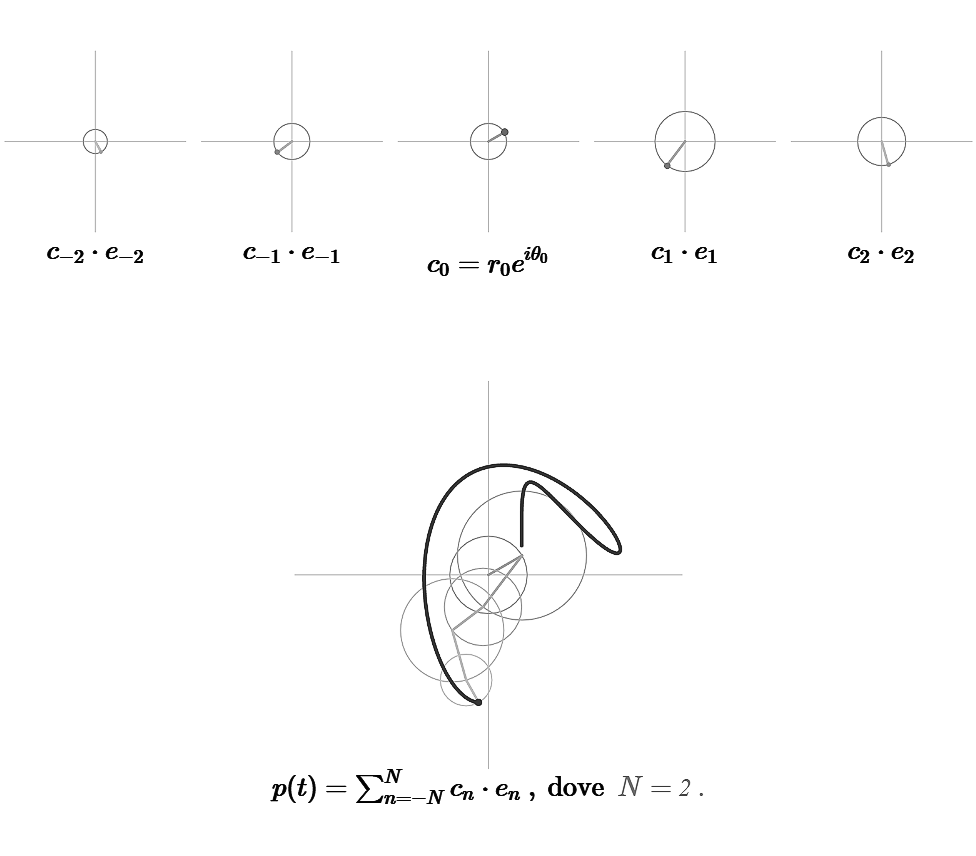
\includegraphics[width=0.8\linewidth]{_images/pol-trig} \end{center}

\begin{itemize}
\tightlist
\item
  Nella \href{https://bradwave.github.io/thesis/\#/animazione-polinomi-trigonometrici-3d}{seconda animazione} è possibile - sempre tramite \emph{rotella del mouse} o \emph{trascinamento verticale} su schermo - rivelare l'asse della variabile \(t\) per mezzo di una rotazione tridimensionale, visualizzando il polinomio trigonometrico nello spazio \(\mathbb{R} \times \mathbb{C}\).
\end{itemize}

\begin{center}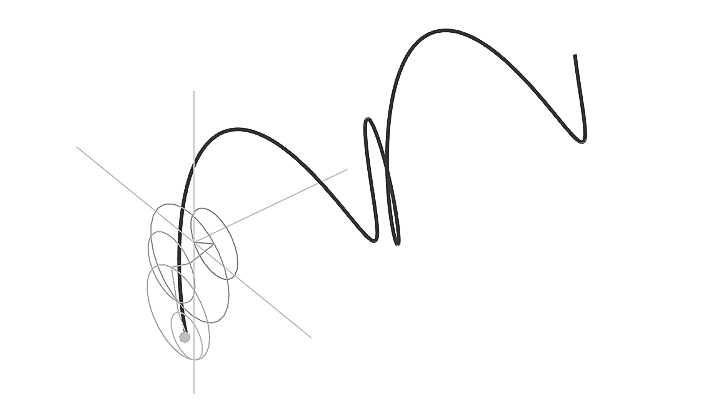
\includegraphics[width=0.5\linewidth]{_images/pol-3d} \end{center}

Introduciamo quindi \(T_n\), spazio vettoriale (di dimensione \(2N-1\)) dei polinomi trigonometrici \(p(t)\) di grado minore o uguale a \(N\), dotato del prodotto scalare
\[(p,q) = \int_{0}^{a} p(t) \overline{q}(t)dt \ .\]
Da \((p,n)=a\cdot c_n\) ricaviamo quindi la \emph{\textbf{formula di Fourier}}

\begin{equation}
  c_n=\frac{1}{a} \int_{0}^{a}p(t)e^{-2 i \pi n \textstyle \frac {t}{a}}dt \ .
  \label{eq:formulafourier}
\end{equation}

Ci poniamo dunque la \textbf{domanda fondamentale}:

\begin{quote}
\emph{se \(f: \mathbb{R} \longrightarrow \mathbb{C} \ \) è una funzione arbitraria di periodo \(a\), possiamo trovare una decomposizione di \(f\) della forma}
\begin{equation}
f(t) = \sum c_n e^{2 \pi in\textstyle \frac{t}{a}} \ ,
\label{eq:domanda}
\end{equation}
\emph{sotto minime ipotesi su \(f\) ?}
\end{quote}

\hypertarget{seriefourier}{%
\section{Segnali periodici e serie di Fourier}\label{seriefourier}}

In un celebre articolo del 1807, \textbf{Joseph Fourier} afferma che la risposta a tale domanda è affermativa, a patto che siano consentite somme infinite.

È possibile ridefinire questa risposta con gli strumenti della matematica moderna.
Per farlo, introduciamo lo spazio
\[L_{p}^2(0,a)= \{ f:\mathbb{R} \longrightarrow \mathbb{C} \ : \ f \ \text{ ha periodo } a \text{ e } \int_{0}^{a}|f(t)|^2dt < +\infty\bigg\}\]

che, dotato delle usuali operazioni, è uno \textbf{spazio vettoriale}. Definiamo quindi il \emph{prodotto scalare}
\[(f,g) = \int_{0}^{a} f(t) \overline{g}(t)dt \ ,\]

e la \emph{norma} associata
\[ \Vert f \Vert_2 = \left( \int_{0}^{a} |f(t)|^2 dt \right) ^{\textstyle \frac{1}{2}} \ .\]
Per rispondere alla \emph{domanda fondamentale} occorre trovare l'elemento \(f_N\) nel sottospazio \(T_n\) di \(L_{p}^{2}(0,a)\) che ha la minima distanza da \(f\). Se esiste, lo chiamiamo la \emph{\textbf{miglior approssimazione}} di \(f\) in \(T_{n}\).
La soluzione è fornita dal seguente teorema:

\begin{quote}
\hypertarget{teorema}{%
\subsubsection*{Teorema}\label{teorema}}
\addcontentsline{toc}{subsubsection}{Teorema}

\emph{Esiste un unico polinomio trigonometrico \(f_N\) in \(T_n\) tale che}
\[ \Vert f - f_N \Vert _{2} = \min_{p \in T_N} \Vert f - p \Vert _{2} \]
\emph{Questo polinomio è dato da}
\begin{equation}
f_{N}(t)=\sum_{n=-N}^{N} c_{n}e^{2\pi in \textstyle \frac {t}{a}} \ ,
\label{eq:polsol}
\end{equation}
\emph{dove}
\begin{equation}
c_n=\frac{1}{a} \int_{0}^{a}f(t)e^{-2 i \pi n \textstyle \frac {t}{a}}dt \ .
\label{eq:coeffsol}
\end{equation}
\end{quote}

Per qualunque \(f \in L_{p}^{2}(0,a) \ \), vale poi la disuguaglianza
\[ \sum_{n=-\infty}^{\infty} |c_n|^{2} < + \infty \]
e quindi
\[ c_n(f) \rightarrow 0 \ \text{ per } \ |n| \rightarrow + \infty \ . \]

Il passaggio successivo consiste nello studio della \textbf{convergenza}.
Grazie ad un \href{https://bradwave.github.io/thesis/\#/esempio-animato}{\textbf{esempio animato}}, è possibile osservare come l'approssimazione, data da una somma di seni, tenda alla funzione \emph{onda quadra}:

\begin{itemize}
\tightlist
\item
  è possibile - tramite \emph{rotella del mouse} o \emph{trascinamento verticale} su schermo - aumentare in numero di addendi nella somma e, quindi, migliorare l'approssimazione.
\end{itemize}

\begin{center}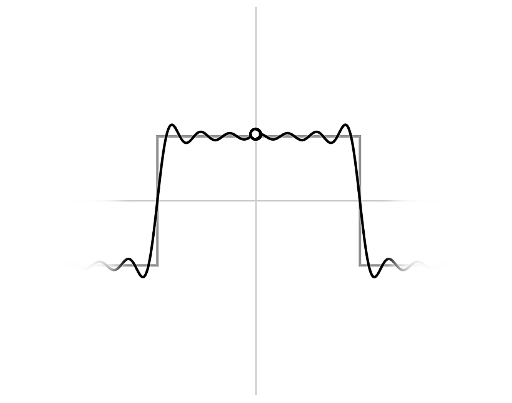
\includegraphics[width=0.5\linewidth]{_images/approx} \end{center}

In conclusione, è possibile scrivere:

\begin{equation}
  f(t) = \sum_{n= - \infty}^{+ \infty} c_n e^{2 i \pi n \textstyle \frac {t}{a}} \ .
  \label{eq:sumeq}
\end{equation}

Si noti che questa è un'equivalenza nella norma di \(L_{p}^{2}(0,a)\) e \textbf{non} significa che, per qualunque valore di \(t\), \(f(t)\) sia uguale alla somma della serie.

\hypertarget{rapprpunt}{%
\section{Rappresentazione puntuale}\label{rapprpunt}}

Poiché una funzione impiegata in \textbf{computazione numeriche} è necessariamente valutata solo in un \textbf{numero finito} di \textbf{punti}, è importante determinare se la formula \eqref{eq:sumeq} possa esprimere un'equivalenza ad un dato punto \(t\).
Questo è il problema della \emph{\textbf{convergenza puntuale}}.

Per risolverlo, ci dovremo estendere oltre \(L^2_p(0,a)\).

Dalla caratterizzazione dell'\emph{\textbf{integrale di Lebesgue}}
\[ f \text{ è Lebesgue-integrabile su } I \ \iff \ \int_{I}|f(t)|dt < +\infty \]
segue immediatamente che i coefficienti di Fourier esistono se e solo se \(f\) è integrabile su \((a,b)\).
Introduciamo la notazione
\[L_{p}^{1}(0,a) = \left\{ f : \mathbb{R} \longrightarrow \mathbb{C} \ : \ f \text{ ha periodo } a  \text{ e } \int_{0}^{a}|f(t)|dt < +\infty \right\} \ .\]
e notiamo che \(L_p^2(0,a) \subset L_p^1(0,a)\), quindi \(f \in L_p^1(0,a)\) è una condizione meno restrittiva di \(f \in L_p^2(0,a)\).

Al momento non sappiamo se la serie \(\sum_{n=-\infty}^{+\infty}c_n(f)e^{2\pi in\frac{t}{a}}\) converga e, in caso di convergenza, non conosciamo il valore del limite.
Una \textbf{condizione necessaria} ma non sufficiente è che \[c_n \rightarrow 0 \text{ per } |n| \rightarrow + \infty \ .\]
Tale condizione è verificata per \(f \in L_p^2(0,a)\) e rimane vera anche per \(f \in L_p^1(0,a)\)

\begin{quote}
\hypertarget{teorema-di-riemann-lebesgue}{%
\subsubsection*{Teorema di Riemann-Lebesgue}\label{teorema-di-riemann-lebesgue}}
\addcontentsline{toc}{subsubsection}{Teorema di Riemann-Lebesgue}

\emph{Sia \((a,b)\) un intervallo limitato e sia \(f\) integrabile su \((a,b)\).}
\emph{Allora l'integrale}
\[ I_n = \int_{a}^{b}f(x)e^{2 \pi in x} dx \rightarrow 0 \ \text{ per } \ |n| \rightarrow + \infty \]
\end{quote}

Un altro importante risultato è riassunto dal \textbf{teorema di Dirichlet}, che mostra come la convergenza della serie di Fourier di \(f\) in un punto \(t_0\) dipende esclusivamente dal \textbf{comportamento} di \(f\) \textbf{in un intorno} di \(t_0\).

\begin{quote}
\hypertarget{teorema-di-dirichlet}{%
\subsubsection*{Teorema di Dirichlet}\label{teorema-di-dirichlet}}
\addcontentsline{toc}{subsubsection}{Teorema di Dirichlet}

\emph{Sia \(f \in L^1_p(0,a)\). Se esistono i limiti \(f(t+)\) e \(f(t-)\) in un punto \(t_0\) ed esistono le derivate destra e sinistra in \(t_0\), allora}
\[f_N(t_0) \rightarrow \frac{1}{2} \big[ f(t_0+) + f(t_0-) \big] \ \text{ per } \ N \rightarrow +\infty \ .\]
\emph{Se \(f\) è continua in \(t_0\), \(f_N(t_0) \rightarrow f(t_0)\).}
\end{quote}

È infine possibile ricavare delle informazioni in merito alla \emph{\textbf{convergenza uniforme}}:

\begin{quote}
\hypertarget{proposizione}{%
\subsubsection*{Proposizione}\label{proposizione}}
\addcontentsline{toc}{subsubsection}{Proposizione}

\emph{Se \(f \in L^2_p(0,a)\) e i suoi coefficienti di Fourier soddisfano}
\[ \sum_{n=-\infty}^{\infty} |c_n| < + \infty \ ,\]
\emph{allora \(f\) è uguale q.o. ad una funzione continua \(\tilde f\) e la serie di Fourier di \(f\) converge uniformemente a \(\tilde f\) su \(\mathbb{R}\).}
\end{quote}

In chiusura, vengono proposte le due animazioni riassuntive che riguardano un \textbf{peculiare esempio}:

\begin{itemize}
\tightlist
\item
  la \href{https://bradwave.github.io/thesis/\#/serie-di-fourier}{prima}, la \textbf{più importante} di tutta la presentazione, mostra la convergenza puntuale alla funzione \(f\) della sua serie di Fourier. È possibile - tramite \emph{rotella del mouse} o \emph{trascinamento verticale} su schermo - migliorare l'approssimazione data dalla somma parziale \(N\)-esima della serie di Fourier, facendo variare \(N\). È inoltre visibile, nella parte superiore, lo \textbf{spettro} del segnale periodico \(f\), definito dall'insieme di coppie \((n/a,c_n), \ n \in \mathbb{Z}\) dove \(c_n\) è l'\(n\)-esimo coefficiente di Fourier di \(f\).
\end{itemize}

\begin{center}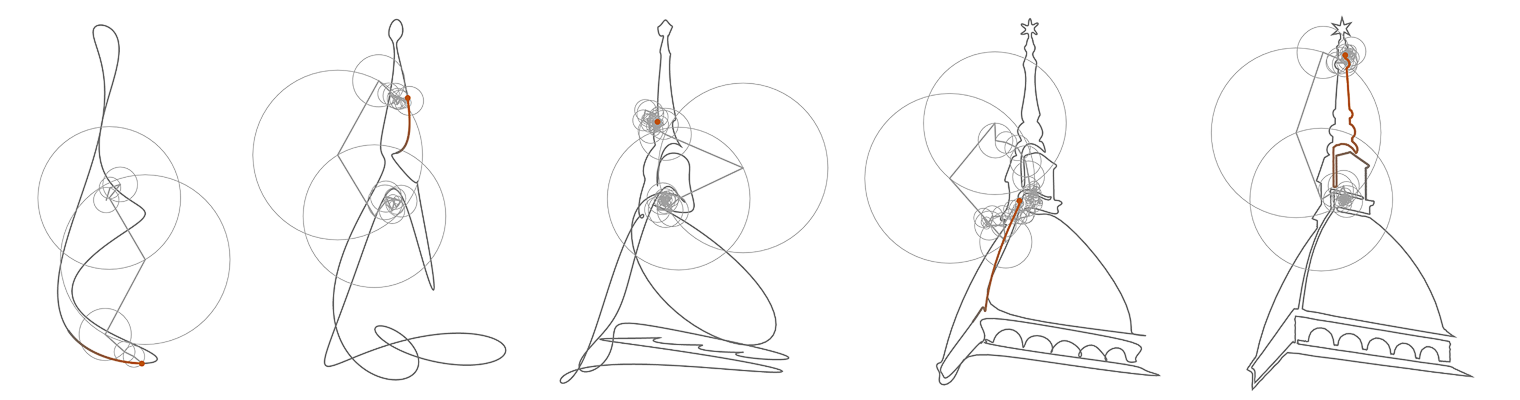
\includegraphics[width=1\linewidth]{_images/serie-fourier} \end{center}

\begin{itemize}
\tightlist
\item
  la \href{https://bradwave.github.io/thesis/\#/scomposizione}{seconda} mette in evidenza, tramite la scomposizione di \(f(t)\) in \(f(t)=u(t)+iv(t)\), la continuità di \(f\) e la sua appartenenza a \(L^1_p(0,a)\);
\end{itemize}

\begin{center}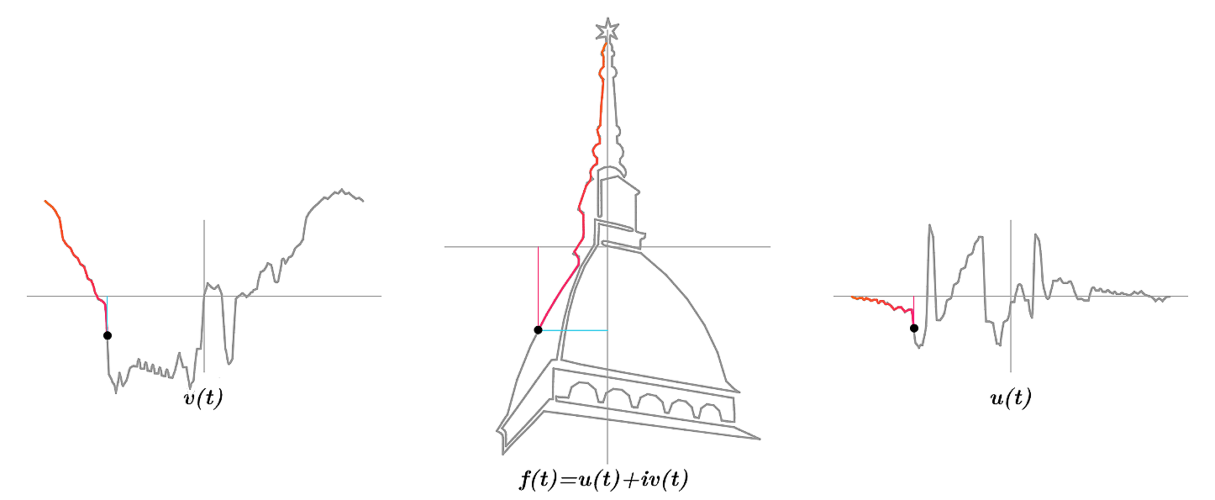
\includegraphics[width=1\linewidth]{_images/decomp} \end{center}

\hypertarget{software}{%
\chapter{Software}\label{software}}

Questo capitolo è dedicato ad una discussione dettagliata di alcune delle più interessanti tecniche informatiche e dei programmi impiegati nella realizzazione della presentazione e delle animazioni.

Il \textbf{codice} è interamente disponibile su \href{https://github.com/Bradwave/thesis}{\emph{\textbf{GitHub}}}.

\hypertarget{softan}{%
\section{Animazioni}\label{softan}}

Le animazioni sono scritte in \emph{JavaScript} e integrate in una pagina HTML. Per facilitare e velocizzare lo sviluppo, ho fatto ampio uso di \href{https://p5js.org/}{\emph{\textbf{p5.js}}}, una libreria grafica \emph{open source} per il \emph{creative coding}, che offre una varietà di funzioni per la rappresentazione di \textbf{costruzioni geometriche}, il \emph{rendering} e la manipolazione del DOM.

Ho inoltre implementato diverse \textbf{funzionalità} per ottimizzare la gestione di alcuni aspetti delle animazioni.

\hypertarget{coordsystem}{%
\subsection{Sistema di coordinate}\label{coordsystem}}

Data la peculiarità del \textbf{sistema di coordinate a schermo} utilizzato da \emph{p5.js} (contraddistinto dall'origine posizionata nell'angolo in alto a sinistra dello schermo e dall'asse \(y\) invertito, come schematizzato in figura) si è reso necessario trovare un \href{https://github.com/Bradwave/thesis/blob/master/animations/js/utils/coordinateSystem.js}{metodo per gestire la conversione} in \textbf{sistema di coordinate cartesiane}. Quest'ultimo viene \textbf{centrato} e \textbf{scalato} in base all'altezza e alla larghezza della finestra contenitore e riconfigurato al ridimensionamento della stessa.

\begin{center}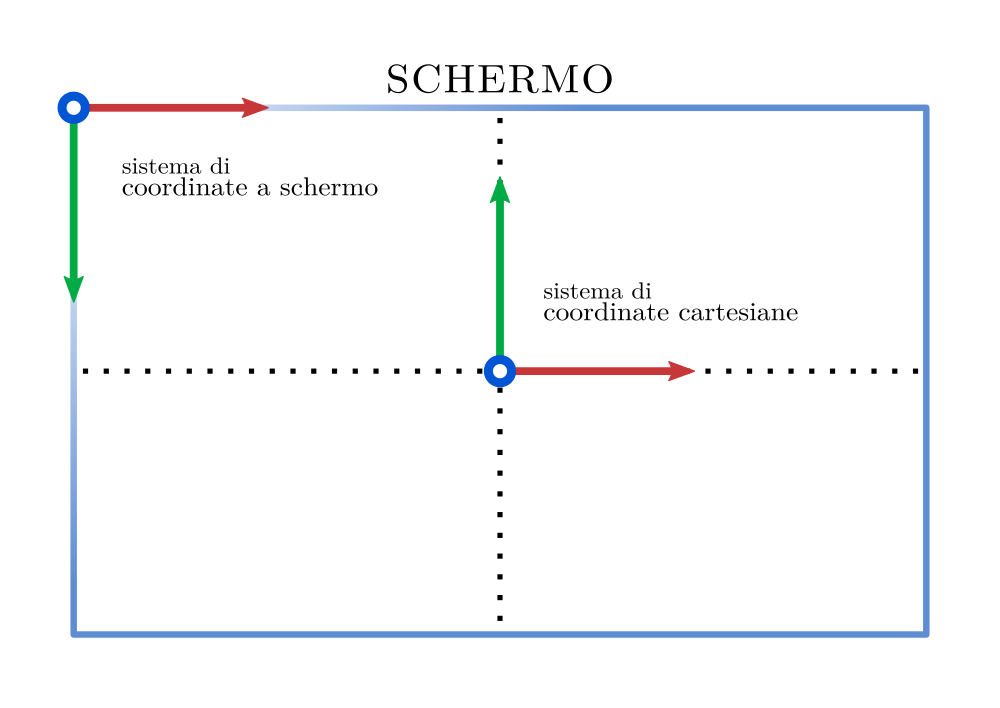
\includegraphics[width=0.6\linewidth]{_images/screen} \end{center}

La funzione \emph{toCartesian} - responsabile della conversione da coordiate a schermo a coordinate cartesiane - tiene conto della dimensione della finestra, informazione contenuta in \emph{descaleFactor}, e della posizione del centro della finestra:

\begin{Shaded}
\begin{Highlighting}[]
\KeywordTok{function} \AttributeTok{toCartesian}\NormalTok{(x}\OperatorTok{,}\NormalTok{ y) }\OperatorTok{\{}
  \KeywordTok{let}\NormalTok{ cx }\OperatorTok{=}\NormalTok{ (x }\OperatorTok{-}\NormalTok{ xOrigin) }\OperatorTok{*}\NormalTok{ descaleFactor}\OperatorTok{;}
  \KeywordTok{let}\NormalTok{ cy }\OperatorTok{=}\NormalTok{ (yOrigin }\OperatorTok{-}\NormalTok{ y) }\OperatorTok{*}\NormalTok{ descaleFactor}\OperatorTok{;}
  \ControlFlowTok{return} \AttributeTok{createVector}\NormalTok{(cx}\OperatorTok{,}\NormalTok{ cy)}\OperatorTok{;}
\OperatorTok{\}}
\end{Highlighting}
\end{Shaded}

Lo stesso vale per la funzione inversa, che converte le coordinate cartesiane in coordinate a schermo:

\begin{Shaded}
\begin{Highlighting}[]
\KeywordTok{function} \AttributeTok{toScreenCoord}\NormalTok{(x}\OperatorTok{,}\NormalTok{ y) }\OperatorTok{\{}
  \KeywordTok{let}\NormalTok{ sx }\OperatorTok{=}\NormalTok{ x }\OperatorTok{*}\NormalTok{ scaleFactor }\OperatorTok{+}\NormalTok{ xOrigin}\OperatorTok{;}
  \KeywordTok{let}\NormalTok{ sy }\OperatorTok{=}\NormalTok{ yOrigin }\OperatorTok{-}\NormalTok{ y }\OperatorTok{*}\NormalTok{ scaleFactor}\OperatorTok{;}
  \ControlFlowTok{return} \AttributeTok{createVector}\NormalTok{(sx}\OperatorTok{,}\NormalTok{ sy)}\OperatorTok{;}
\OperatorTok{\}}
\end{Highlighting}
\end{Shaded}

\hypertarget{progrbar}{%
\subsection{Barra del progresso}\label{progrbar}}

La \href{https://github.com/Bradwave/thesis/blob/master/animations/js/utils/progressGraphics.js}{\textbf{barra del progresso}} (o \emph{progress bar}) è un importante strumento di \textbf{accessibilità} e restituisce un \emph{feedback} in merito al progresso possibile nell'interazione da parte dell'utente con l'animazione. La barra è posizionata sul lato destro dello schermo e monitora il comportamento dell'utente, attivandosi solo durante un'interazione e scomparendo dopo qualche secondo, per non interferire con il resto dell'animazione.

È inoltre accompagnata da un'\textbf{icona} di un \textbf{mouse}, da me disegnata, che comunica all'utente, con delle apposite frecce pulsati, le azioni possibili.

\hypertarget{anserie}{%
\subsection{La serie di Fourier}\label{anserie}}

Per rappresentare la serie di Fourier di una funzione periodica \(f(t)\) occorre \textbf{definire} con precisione la \textbf{funzione} - in modo che sia anche semplice da replicare graficamente - e calcolarne i \textbf{coefficienti di Fourier}.

\hypertarget{polbezier}{%
\subsubsection{Polybézier}\label{polbezier}}

Il mezzo ideale per definire la funzione \(f(t)\) si è rivelato essere la \emph{polybézier}.

Una \textbf{\emph{polybézier}}, o curva di Bézier composta, è una \textbf{curva di Bézier} definita a tratti e continua, vale a dire una concatenazione di curve di Bézier. In particolare, si prenderà in esame il caso di una concatenazione di curve di Bézier \textbf{cubiche}, ovvero il tracciato percorso dalla curva di parametrizzazione

\begin{equation}
    \mathbf{B}(t)=\mathbf{P}_0(1-t)^3+3\mathbf{P}_1t(1-t)^2+2\mathbf{P}_2t^2(1-t)+\mathbf{P}_3t^3 \ , \ t \in [0,1] \ .
    \label{eq:bezier}
\end{equation}

La curva passa per i punti \(\mathbf{P}_0\) e \(\mathbf{P}_3\), ma non per i punti \(\mathbf{P}_1\) e \(\mathbf{P}_2\) che sono di \emph{controllo} e forniscono informazioni direzionali. Il modo più semplice per comprendere la sua natura è visualizzarla:

\begin{center}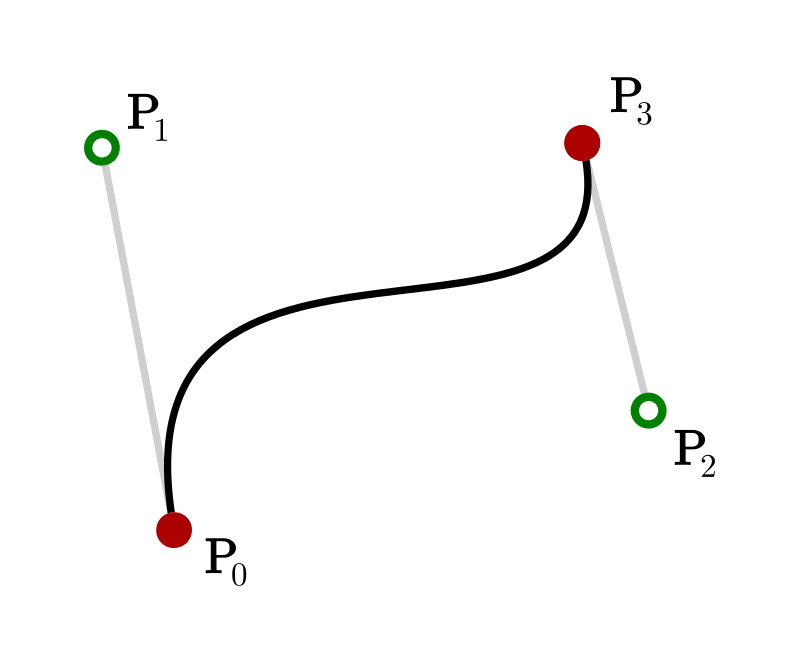
\includegraphics[width=0.36\linewidth]{_images/bezier} \end{center}

Una \emph{polybézier} cubica è formata da un numero \(M \in \mathbb{N}\) di curve \(\mathbf{B}^j(t), \ t \in [0,1], \ j=0,...,M-1\) tali che \(\mathbf{B}^j(1)=\mathbf{B}^{j+1}(0)\). La curva risulterà chiusa se \(\mathbf{B}^0(0)=\mathbf{B}^{M-1}(1)\).

\begin{center}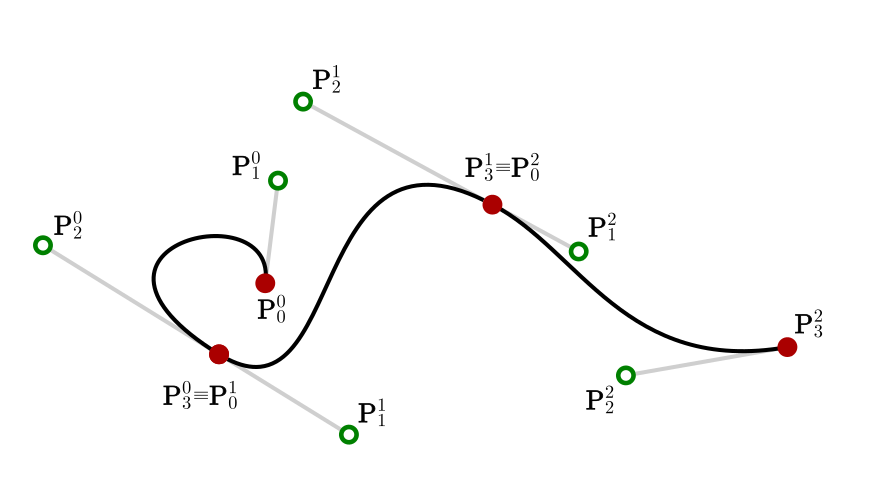
\includegraphics[width=0.75\linewidth]{_images/polybezier} \end{center}

Ho disegnato le curve con \href{https://inkscape.org/}{\emph{\textbf{Inkscape}}}, un editor grafico vettoriale \emph{open source}. Il file generato - di formato SVG - può essere aperto con un semplice editor di testo e, al suo interno, ho identificato le coordinate dei punti. Ho poi scritto delle \href{https://github.com/Bradwave/thesis/blob/master/animations/js/utils/polybezier.js}{funzioni \emph{JavaScript}} per trasformare una stringa testuale in coordinate numeriche, \textbf{trovare le coordinate} di un punto \(\mathbf{P}(t)\) giacente sulla curva dato \(t\)

\begin{Shaded}
\begin{Highlighting}[]
\AttributeTok{getPoint}\NormalTok{(p0}\OperatorTok{,}\NormalTok{ p1}\OperatorTok{,}\NormalTok{ p2}\OperatorTok{,}\NormalTok{ p3}\OperatorTok{,}\NormalTok{ t) }\OperatorTok{\{}
  \KeywordTok{let}\NormalTok{ x }\OperatorTok{=} \VariableTok{p0}\NormalTok{.}\AttributeTok{x} \OperatorTok{*} \AttributeTok{pow}\NormalTok{(}\DecValTok{1} \OperatorTok{-}\NormalTok{ t}\OperatorTok{,} \DecValTok{3}\NormalTok{) }\OperatorTok{+} \DecValTok{3} \OperatorTok{*} \VariableTok{p1}\NormalTok{.}\AttributeTok{x} \OperatorTok{*}\NormalTok{ t }\OperatorTok{*} \AttributeTok{pow}\NormalTok{(}\DecValTok{1} \OperatorTok{-}\NormalTok{ t}\OperatorTok{,} \DecValTok{2}\NormalTok{)}
    \OperatorTok{+} \DecValTok{3} \OperatorTok{*} \VariableTok{p2}\NormalTok{.}\AttributeTok{x} \OperatorTok{*} \AttributeTok{pow}\NormalTok{(t}\OperatorTok{,} \DecValTok{2}\NormalTok{) }\OperatorTok{*}\NormalTok{ (}\DecValTok{1} \OperatorTok{-}\NormalTok{ t) }\OperatorTok{+} \VariableTok{p3}\NormalTok{.}\AttributeTok{x} \OperatorTok{*} \AttributeTok{pow}\NormalTok{(t}\OperatorTok{,} \DecValTok{3}\NormalTok{)}\OperatorTok{;}
  \KeywordTok{let}\NormalTok{ y }\OperatorTok{=} \VariableTok{p0}\NormalTok{.}\AttributeTok{y} \OperatorTok{*} \AttributeTok{pow}\NormalTok{(}\DecValTok{1} \OperatorTok{-}\NormalTok{ t}\OperatorTok{,} \DecValTok{3}\NormalTok{) }\OperatorTok{+} \DecValTok{3} \OperatorTok{*} \VariableTok{p1}\NormalTok{.}\AttributeTok{y} \OperatorTok{*}\NormalTok{ t }\OperatorTok{*} \AttributeTok{pow}\NormalTok{(}\DecValTok{1} \OperatorTok{-}\NormalTok{ t}\OperatorTok{,} \DecValTok{2}\NormalTok{)}
    \OperatorTok{+} \DecValTok{3} \OperatorTok{*} \VariableTok{p2}\NormalTok{.}\AttributeTok{y} \OperatorTok{*} \AttributeTok{pow}\NormalTok{(t}\OperatorTok{,} \DecValTok{2}\NormalTok{) }\OperatorTok{*}\NormalTok{ (}\DecValTok{1} \OperatorTok{-}\NormalTok{ t) }\OperatorTok{+} \VariableTok{p3}\NormalTok{.}\AttributeTok{y} \OperatorTok{*} \AttributeTok{pow}\NormalTok{(t}\OperatorTok{,} \DecValTok{3}\NormalTok{)}\OperatorTok{;}
  \ControlFlowTok{return} \KeywordTok{new} \AttributeTok{Complex}\NormalTok{(x}\OperatorTok{,}\NormalTok{ y)}\OperatorTok{;}
\OperatorTok{\}}
\end{Highlighting}
\end{Shaded}

e infine \textbf{campionare \(N\) punti} lungo la \emph{polybézier}, \textbf{distanziati equamente} nella variabile \(t \in [0,1]\):

\begin{Shaded}
\begin{Highlighting}[]
\AttributeTok{samplePoints}\NormalTok{(N) }\OperatorTok{\{}
  \KeywordTok{let}\NormalTok{ s }\OperatorTok{=} \FloatTok{1.000000} \OperatorTok{/}\NormalTok{ N}\OperatorTok{;}
  \KeywordTok{let}\NormalTok{ M }\OperatorTok{=} \KeywordTok{this}\NormalTok{.}\VariableTok{points}\NormalTok{.}\AttributeTok{length} \OperatorTok{/} \DecValTok{3}\OperatorTok{;}
  \KeywordTok{let}\NormalTok{ sampledPoints }\OperatorTok{=}\NormalTok{ []}\OperatorTok{;}
  
  \ControlFlowTok{for}\NormalTok{ (}\KeywordTok{let}\NormalTok{ j }\OperatorTok{=} \DecValTok{0}\OperatorTok{;}\NormalTok{ j }\OperatorTok{<}\NormalTok{ M}\OperatorTok{;}\NormalTok{ j}\OperatorTok{++}\NormalTok{) }\OperatorTok{\{}
    \KeywordTok{let}\NormalTok{ points }\OperatorTok{=} \OperatorTok{\{}
      \DataTypeTok{p0}\OperatorTok{:} \KeywordTok{this}\NormalTok{.}\AttributeTok{points}\NormalTok{[}\DecValTok{3} \OperatorTok{*}\NormalTok{ j]}\OperatorTok{,} \DataTypeTok{p1}\OperatorTok{:} \KeywordTok{this}\NormalTok{.}\AttributeTok{points}\NormalTok{[}\DecValTok{1} \OperatorTok{+} \DecValTok{3} \OperatorTok{*}\NormalTok{ j]}\OperatorTok{,}
      \DataTypeTok{p2}\OperatorTok{:} \KeywordTok{this}\NormalTok{.}\AttributeTok{points}\NormalTok{[}\DecValTok{2} \OperatorTok{+} \DecValTok{3} \OperatorTok{*}\NormalTok{ j]}\OperatorTok{,} \DataTypeTok{p3}\OperatorTok{:} \KeywordTok{this}\NormalTok{.}\AttributeTok{points}\NormalTok{[(}\DecValTok{3} \OperatorTok{+} \DecValTok{3} \OperatorTok{*}\NormalTok{ j)}
        \OperatorTok{%} \KeywordTok{this}\NormalTok{.}\VariableTok{points}\NormalTok{.}\AttributeTok{length}\NormalTok{]}
    \OperatorTok{\};}
    \ControlFlowTok{for}\NormalTok{ (}\KeywordTok{let}\NormalTok{ k }\OperatorTok{=} \DecValTok{0}\OperatorTok{;}\NormalTok{ k }\OperatorTok{<}\NormalTok{ N}\OperatorTok{;}\NormalTok{ k}\OperatorTok{++}\NormalTok{) }\OperatorTok{\{}
\NormalTok{      sampledPoints[k }\OperatorTok{+}\NormalTok{ j }\OperatorTok{*}\NormalTok{ N] }\OperatorTok{=} \KeywordTok{this}\NormalTok{.}\AttributeTok{getPoint}\NormalTok{(}\VariableTok{points}\NormalTok{.}\AttributeTok{p0}\OperatorTok{,}
        \VariableTok{points}\NormalTok{.}\AttributeTok{p1}\OperatorTok{,} \VariableTok{points}\NormalTok{.}\AttributeTok{p2}\OperatorTok{,} \VariableTok{points}\NormalTok{.}\AttributeTok{p3}\OperatorTok{,}\NormalTok{ k }\OperatorTok{*}\NormalTok{ s)}\OperatorTok{;}
    \OperatorTok{\}}
  \OperatorTok{\}}
  \ControlFlowTok{return}\NormalTok{ sampledPoints}\OperatorTok{;}
\OperatorTok{\}}
\end{Highlighting}
\end{Shaded}

\hypertarget{dft}{%
\subsection{La trasformata discreta di Fourier}\label{dft}}

Non potendo computare esplicitamente i \textbf{coefficienti di Fourier} con l'integrale
\[ c_n=\frac{1}{a} \int_{0}^{a}f(t)e^{-2 i \pi n \textstyle \frac {t}{a}}dt \ , \]
sono ricorso alla \textbf{trasformata discreta di Fourier}.
Per farlo, è necessario assumere che la funzione \(f(t)\), di cui si vogliono calcolare i coefficienti, sia periodica di periodo \(a\) e che \(N\) dei suoi valori siano equamente distanziati sul periodo:

\[f \bigg( k\frac{a}{N} \bigg)=y_{k} \ , \ \ k=0,1,2,..., N-1 \ .\]
Pertanto, si assume che il segnale \(f(t)\) sia campionato a tempi equamente distanziati di \(\frac{a}{N}\) unità.
Si assume inoltre che la serie di Fourier converga puntualmente a \(f\) e che nei punti di discontinuità

\[f(t)=\frac{1}{2}\big(f(t+)+f(t-)\big) \ .\]

Con la \emph{formula del trapezio}, si ottiene un'\textbf{approssimazione} dei coefficienti di Fourier della funzione \(f\):

\begin{equation}
    c'_n=\frac{1}{N}\sum_{k=0}^{N-1}y_{k}e^{-2\pi in\frac{k}{N}}
    \label{eq:dcoeff}
\end{equation}

Tradotto in termini informatici, la \href{https://github.com/Bradwave/thesis/blob/master/animations/js/utils/fourier.js}{funzione responsabile} del computo della trasformata discreta può essere così espressa:

\begin{Shaded}
\begin{Highlighting}[]
\KeywordTok{function} \AttributeTok{dft}\NormalTok{(y) }\OperatorTok{\{}
  \KeywordTok{const}\NormalTok{ Y }\OperatorTok{=}\NormalTok{ []}\OperatorTok{;}
  \KeywordTok{const}\NormalTok{ N }\OperatorTok{=} \VariableTok{y}\NormalTok{.}\AttributeTok{length}\OperatorTok{;}
  
  \ControlFlowTok{for}\NormalTok{ (}\KeywordTok{let}\NormalTok{ n }\OperatorTok{=} \DecValTok{0}\OperatorTok{;}\NormalTok{ n }\OperatorTok{<}\NormalTok{ N}\OperatorTok{;}\NormalTok{ n}\OperatorTok{++}\NormalTok{) }\OperatorTok{\{}
    \KeywordTok{let}\NormalTok{ sum }\OperatorTok{=} \KeywordTok{new} \AttributeTok{Complex}\NormalTok{(}\DecValTok{0}\OperatorTok{,} \DecValTok{0}\NormalTok{)}\OperatorTok{;}
    \ControlFlowTok{for}\NormalTok{ (}\KeywordTok{let}\NormalTok{ k }\OperatorTok{=} \DecValTok{0}\OperatorTok{;}\NormalTok{ k }\OperatorTok{<}\NormalTok{ N}\OperatorTok{;}\NormalTok{ k}\OperatorTok{++}\NormalTok{) }\OperatorTok{\{}
      \KeywordTok{const}\NormalTok{ phi }\OperatorTok{=}\NormalTok{ (}\OperatorTok{-}\NormalTok{ TWO_PI }\OperatorTok{*}\NormalTok{ k }\OperatorTok{*}\NormalTok{ n) }\OperatorTok{/}\NormalTok{ N}\OperatorTok{;}
      \KeywordTok{const}\NormalTok{ c }\OperatorTok{=} \KeywordTok{new} \AttributeTok{Complex}\NormalTok{(}\AttributeTok{cos}\NormalTok{(phi)}\OperatorTok{,} \AttributeTok{sin}\NormalTok{(phi))}\OperatorTok{;}
      \VariableTok{sum}\NormalTok{.}\AttributeTok{add}\NormalTok{(y[k].}\AttributeTok{mult}\NormalTok{(c))}\OperatorTok{;}
    \OperatorTok{\}}
\NormalTok{    sum }\OperatorTok{=} \VariableTok{sum}\NormalTok{.}\AttributeTok{div}\NormalTok{(N)}\OperatorTok{;}

    \KeywordTok{let}\NormalTok{ freq }\OperatorTok{=}\NormalTok{ n}\OperatorTok{;}
    \KeywordTok{let}\NormalTok{ amp }\OperatorTok{=} \VariableTok{sum}\NormalTok{.}\AttributeTok{amp}\NormalTok{()}\OperatorTok{;}
    \KeywordTok{let}\NormalTok{ phase }\OperatorTok{=} \VariableTok{sum}\NormalTok{.}\AttributeTok{phase}\NormalTok{()}\OperatorTok{;}
    
\NormalTok{    Y[n] }\OperatorTok{=} \OperatorTok{\{}\NormalTok{ freq}\OperatorTok{,}\NormalTok{ amp}\OperatorTok{,}\NormalTok{ phase }\OperatorTok{\};}
  \OperatorTok{\}}
  
  \ControlFlowTok{return}\NormalTok{ Y}\OperatorTok{;}
\OperatorTok{\}}
\end{Highlighting}
\end{Shaded}

Applicando questo risultato ad una \protect\hyperlink{polbezier}{\emph{polybézier}} chiusa e composta da \(M\) curve di Bézier cubiche \(\mathbf{B}^j(t), \ t \in [0,1], \ j=0,...,M-1\), si ottiene:

\begin{equation}
    c'_n=\frac{1}{M\cdot N'}\sum_{j=0}^{M-1}\sum_{k=0}^{N'-1}\mathbf{B}^{j}\bigg(\frac{k}{N'}\bigg)e^{-2\pi in \textstyle \frac{j\cdot N'+ k}{M\cdot N}}
    \label{eq:beziercoeff}
\end{equation}

dove \(N'\) è il numero di punti campionati per ogni curva di Bézier che compone la \emph{polybébezier}.

\hypertarget{rapprserie}{%
\subsection{La rappresentazione della serie di Fourier}\label{rapprserie}}

Data la funzione \(f(t)\), ovvero la \emph{polybézier}, e i coefficienti della serie di Fourier associata, computati con una trasformata discreta di Fourier, si può procedere alla \textbf{rappresentazione grafica} della serie. Una funzione si occupa di calcolare i punti del percorso tracciato al variare del tempo (\emph{time} \(\in [0,2\pi]\)) e dati \emph{N} coefficienti:

\begin{Shaded}
\begin{Highlighting}[]
\KeywordTok{function} \AttributeTok{epicycles}\NormalTok{(time) }\OperatorTok{\{}
  \KeywordTok{let}\NormalTok{ N }\OperatorTok{=} \VariableTok{fourier}\NormalTok{.}\AttributeTok{length}\OperatorTok{;}
  
  \KeywordTok{let}\NormalTok{ x }\OperatorTok{=} \DecValTok{0}\OperatorTok{;}
  \KeywordTok{let}\NormalTok{ y }\OperatorTok{=} \DecValTok{0}\OperatorTok{;}

  \ControlFlowTok{for}\NormalTok{ (}\KeywordTok{let}\NormalTok{ n }\OperatorTok{=} \DecValTok{0}\OperatorTok{;}\NormalTok{ n }\OperatorTok{<}\NormalTok{ N}\OperatorTok{;}\NormalTok{ n}\OperatorTok{++}\NormalTok{) }\OperatorTok{\{}
    \KeywordTok{let}\NormalTok{ prevx }\OperatorTok{=}\NormalTok{ x}\OperatorTok{;}
    \KeywordTok{let}\NormalTok{ prevy }\OperatorTok{=}\NormalTok{ y}\OperatorTok{;}

    \KeywordTok{let}\NormalTok{ freq }\OperatorTok{=}\NormalTok{ fourier[n].}\AttributeTok{freq}\OperatorTok{;}
    \KeywordTok{let}\NormalTok{ radius }\OperatorTok{=}\NormalTok{ fourier[n].}\AttributeTok{amp}\OperatorTok{;}
    \KeywordTok{let}\NormalTok{ phase }\OperatorTok{=}\NormalTok{ fourier[n].}\AttributeTok{phase}\OperatorTok{;}

\NormalTok{    x }\OperatorTok{+=}\NormalTok{ radius }\OperatorTok{*} \AttributeTok{cos}\NormalTok{(freq }\OperatorTok{*}\NormalTok{ time }\OperatorTok{+}\NormalTok{ phase)}\OperatorTok{;}
\NormalTok{    y }\OperatorTok{+=}\NormalTok{ radius }\OperatorTok{*} \AttributeTok{sin}\NormalTok{(freq }\OperatorTok{*}\NormalTok{ time }\OperatorTok{+}\NormalTok{ phase)}\OperatorTok{;}

    \AttributeTok{ellipse}\NormalTok{(prevx}\OperatorTok{,}\NormalTok{ prevy}\OperatorTok{,}\NormalTok{ radius }\OperatorTok{*} \DecValTok{2}\NormalTok{)}\OperatorTok{;}
    \AttributeTok{line}\NormalTok{(prevx}\OperatorTok{,}\NormalTok{ prevy}\OperatorTok{,}\NormalTok{ x}\OperatorTok{,}\NormalTok{ y)}\OperatorTok{;}
  \OperatorTok{\}}
  
  \ControlFlowTok{return} \AttributeTok{createVector}\NormalTok{(x}\OperatorTok{,}\NormalTok{ y)}\OperatorTok{;}
\OperatorTok{\}}
\end{Highlighting}
\end{Shaded}

I \textbf{punti} sono quindi \textbf{salvati} in un vettore (\emph{path}) e \textbf{uniti} per formare il percorso:

\begin{Shaded}
\begin{Highlighting}[]
    
\end{Highlighting}
\end{Shaded}

\hypertarget{pressoft}{%
\section{Presentazione}\label{pressoft}}

Come già spiegato in un \protect\hyperlink{presentazione}{precedente capitolo}, le slide sono state create attraverso il \emph{framework} per presentazioni HTML \href{https://revealjs.com/}{\emph{\textbf{Reveal.js}}}, modificato e \textbf{personalizzato} per meglio adattarsi alla \protect\hyperlink{filosofia}{visione artistica} generale del progetto. \emph{Reveal.js} permette di scrivere la presentazione usando il noto linguaggio di \emph{markup} HTML. Questo approccio offre numerosi vantaggi: la \emph{portabilità} del file su molti dispositivi, la compattezza del file e la possibilità di una semplice diffusione online.
Inoltre, l'aspetto estetico può essere controllato tramite un \href{https://github.com/Bradwave/thesis/blob/master/dist/theme/math.css}{apposito \emph{style sheet} CSS} in modo rapido e preciso.

La scelta è ricaduta su questo approccio per la necessità di \textbf{integrare fluidamente} le animazioni. \emph{Reveal.js} consente infatti di visualizzare pagine web sullo sfondo delle slide; ciò mi ha permesso di collegare i file HTML contententi le animazioni.

\begin{Shaded}
\begin{Highlighting}[]
\CommentTok{<!-- Convergenza -->}
\KeywordTok{<section}
\OtherTok{  data-background-iframe=}\StringTok{"https://bradwave.github.io/thesis/animations/s4-animation.html"}
\OtherTok{	data-preload data-auto-animate}\KeywordTok{>}
	\KeywordTok{<h4>}\NormalTok{2.2.1 Convergenza dell'approssimazione $ $}\KeywordTok{</h4>}
	\KeywordTok{<hr>}
	\KeywordTok{<p>}
\NormalTok{		Cosa succede a $f_N$ per $N \textbackslash{}rightarrow + \textbackslash{}infty$ ?}
	\KeywordTok{</p>}
	
\NormalTok{	...}
	
\KeywordTok{</section>}
\end{Highlighting}
\end{Shaded}

Come visibile in questo esempio, l'attributo \emph{data-background-iframe} definisce il link all'animzione; il titolo della slide è contenuto in un \emph{header}, il testo nei paragrafi e il \emph{blockquote} racchiude invece il testo dell'esempio. La classe \emph{fragment} consente invece la comparsa graduale degli elementi.

Le formule matematiche vengono visualizzate grazie al \emph{display engine} \href{https://www.mathjax.org/}{\emph{\textbf{MathJax}}}.

\hypertarget{bibliografia}{%
\chapter*{Bibliografia}\label{bibliografia}}
\addcontentsline{toc}{chapter}{Bibliografia}

\begin{enumerate}
\def\labelenumi{\arabic{enumi}.}
\tightlist
\item
  C. Gasquet e P. Witomksi, \emph{Fourier Analysis and Applications}, 1a ed., New York, NY, Springer, 1999.
\item
  3Blue1Brown, \href{www.youtube.com/watch?v=r6sGWTCMz2k}{\emph{But what is a Fourier series? From heat flow to circle drawings}}, su \href{https://www.youtube.com}{YouTube}, 2019.
\item
  Pomax, \href{https://pomax.github.io/bezierinfo/\#polybezier}{\emph{A Primer on Bézier Curves}}, su \href{https://github.com/}{github.com}, accesso nel 2020.
\item
  W. Rudin, \emph{Real and Complex Analysis}, Singapore, McGraw Hill Book Co, 1987.
\item
  E. Oran Briigham, \emph{The FFT and its Applications}, Englewood Clifs, Prentice-Hall, 1988.
\item
  S. W. Smith, \emph{The Scientist and Engineer's Guide to Digital Signal Processing}, California Technical Pub, 1997.
\item
  O. Byrne, \emph{The First Six Books of Euclid}, Londra, William Pickering, 1847.
\end{enumerate}

\hypertarget{documentazione}{%
\subsubsection*{Documentazioni}\label{documentazione}}
\addcontentsline{toc}{subsubsection}{Documentazioni}

\begin{enumerate}
\def\labelenumi{\arabic{enumi}.}
\setcounter{enumi}{7}
\tightlist
\item
  \emph{p5.js}, su \href{https://p5js.org}{p5js.org}
\item
  \emph{reveal.js}, su \href{https://revealjs.com}{revealjs.com}
\item
  \emph{Complex.js}, su \href{https://github.com/infusion/Complex.js}{github.com/infusion/Complex.js/}
\item
  \emph{MathJax}, su \href{https://www.mathjax.org/}{www.mathjax.org}
\item
  \href{https://math.meta.stackexchange.com/questions/5020/mathjax-basic-tutorial-and-quick-reference}{\emph{MathJax basic tutorial and quick reference}}, su \href{https://math.meta.stackexchange.com/}{math.meta.stackexchange.com/}
\end{enumerate}

\begin{enumerate}
\def\labelenumi{\arabic{enumi}.}
\setcounter{enumi}{12}
\tightlist
\item
  Y. Xie, \href{https://bookdown.org/yihui/bookdown/}{\emph{Bookdown: Authoring Books and Technical Documents with R Markdown}}, 2020.
\item
  Y. Xie, \emph{Bookdown: Authoring Books and Technical Documents with R Markdown}, Boca Raton, Florida, Chapman e Hall/CRC, 2016
\item
  Y. Xie, J. J. Allaire e G. Grolemund, \emph{R markdown: The definitive guide}, Boca Raton, Florida, Chapman e Hall/CRC, 2018.
\end{enumerate}

\end{document}
